\section{Conclusion and Future Work}
In this chapter we provided the details of how a swarm of UAVs can be used to gather data in a given region described by a polygon. We described how to discretise the region into a set of grid points and we implemented a Nearest Neighbor (NN) heuristic algorithm to generate routes for the swarm of UAVs which visit each grid point in the region exactly once, which is a solution to the multiple Travelling Salesman Problem. For practical purposes in relation to ROCSAFE \cite{rocsafeNUIG}, the project that has funded this work, this solved the surveying problem. The tests carried out in simulation were carried out successfully, using the user interface and custom simulation environment, illustrated in \ref{fig:VirtualPlannedRoutes}, which offers some validation to the work. We then extended this work to use a linear program solver, as proposed in the literature. We managed to prototype a solution using the OR-Tools code repository <provide link>.

The OR-Tools solution is highly flexible, allowing the user to specify arbitrary charging locations, battery capacities, sampling times, optional enforced start and finish locations, operational speeds, etc. However, for the small-scale grids explored, the average solution took x seconds to compute, which indicates that the implemented solution may not scale well. We outline how this may be overcome in the future work section.

Since we were limited by time constraints with this work, we outline some future work that we planned but did not have the time to execute.\par

\subsubsection{Future Work}
We describe some future work that could be done to build on the basic solutions to the problem of finding a scalable solution to the mTSP and VRP described in this chapter. The points outlined are all taken to be specific to the Euclidean grid-based approach that was discussed throughout this chapter.

\begin{enumerate}
    \item The NN solution offered a method that could provide qualitatively good solutions in many scenarios 
    
    \item The quality of the solution to the TSP given by the NN algorithm is known to be dependent on the start position <suitable reference missing>. A common improvement to the algorithm is to run it $n$ times for each possible starting point at each node in the network of $n$ nodes, and then take the best solution found. In the case of the mTSP, for $k$ UAVs, this would mean exploring ${n \choose k}$ different combinations of starting positions, which may make the running time of the algorithm prohibitively long. Therefore, future research could explore an effective way of determining the best starting nodes for the UAVs without implementing a brute force search to improve the NN solution.
    \item Many solutions to the mTSP problem use \textit{iterative improvement} strategies,  which use an existing algorithm to create a solution, then have another algorithm improve the solution.\textit{ Ensemble} strategies are also frequently used, which applies a set of algorithms to the  problem and returns the best solution. The use of either of these techniques with the NN algorithm could provide significantly better results, especially given that this has been shown in the case of Euclidean distance cost functions. For example, reversing some segments that "cross" guarantees an improvement via the \textit{triangle inequality}, as shown in Figure \ref{fig:fixingTourCrossing}. 
    \item Many open-source and commercial linear program solvers exist which are optimized to deal with the mTSP and VRP. We discussed how we used Google's OR-Tools repository <link in footnote> to prototype a solution. Future work could involve optimising the configuration of the problem and choice of back-end solver to produce a scalable solution.
    \item Representing the problem in a different manner may yield a suitable solution that is easier to computer. For example, representing the region to survey as continuous space rather than a discrete grid may facilitate the development of a control algorithm that is simpler and more effective in solving the surveying problem than the ones that exist that deal with discrete grids.
    \item Further theoretical analysis of the algorithm performance could yield insight in how to improve it. Given that it solves some instances of the problem with good results, e.g. that of Figure \ref{table:NNAlgoResultsRect}, the simple, scalable NN solution could be modified to deal with more general problems by using a divide-and-conquer approach to smaller rectangular regions.
    \item UAVs may be unreliable and the assumptions of deterministic sampling times and transition times between locations are not valid in real-world application. A decentralized algorithm which can handle this inherent stochastic element would provide a more robust solution to the surveying problem using multiple UAVs, which could be far superior to the solution presented in this thesis.
    
    
\end{enumerate}


\begin{figure}
\centering
\begin{minipage}{.5\textwidth}
  \centering
  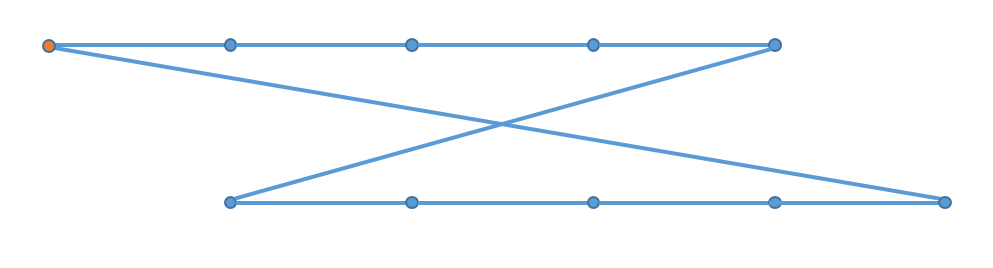
\includegraphics[width=.48\linewidth]{Chapters/MultiAgentCoverage/Figs/crossingSegments.PNG}
  \captionof*{figure}{"X" present in a tour}
  \label{fig:crossingTour}
\end{minipage}%
\begin{minipage}{.5\textwidth}
  \centering
  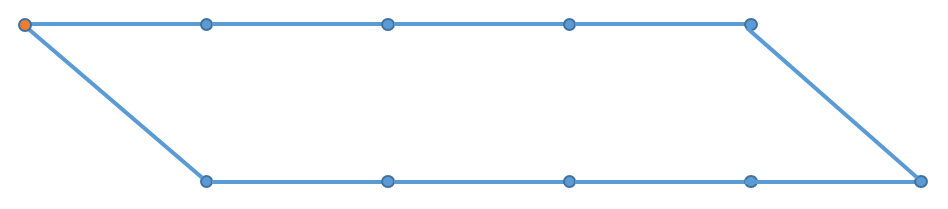
\includegraphics[width=.48\linewidth]{Chapters/MultiAgentCoverage/Figs/nonCrossingSegments.png}
  \captionof*{figure}{"X" removed from tour by reversing segments}
  \label{fig:nonCrossingTour}
\end{minipage}
\caption{Using the triangle inequality to improve tours.}
%Figures based on those found in \href{https://github.com/norvig/pytudes/blob/master/ipynb/TSP.ipynb}{Norvig's TSP github repo.}}
%\footnote{\href {https://github.com/norvig/pytudes/blob/master/ipynb/TSP.ipynb}{https://github.com/norvig/pytudes/blob/master/ipynb/TSP.ipynb}}
\label{fig:fixingTourCrossing}
\end{figure}
%\footnote{\href {https://github.com/norvig/pytudes/blob/master/ipynb/TSP.ipynb}{https://github.com/norvig/pytudes/blob/master/ipynb/TSP.ipynb}}























